\documentclass[12pt]{article}
\usepackage{setspace, graphicx, fullpage, amssymb, amsmath, epsfig, natbib, array, multirow, hyperref}
\usepackage{amsfonts, bm} 
\usepackage{dcolumn}
\usepackage{subfigure, float} 
\usepackage[margin=.5in]{geometry} 
\usepackage{verbatim}
\usepackage{url}
\usepackage{enumerate}
\newcolumntype{d}[1]{D{.}{.}{#1}} 

\begin{document}
	
	\begin{center}
		Update: 07 December 2016
	\end{center}

Due to errors in our code which have since been resolved, the sorting algorithms which include simulated annealing and random reassignment of votes that have changed designation twice in a row (what we have referred to as the hybrid model, typically) is still running as I am writing this update. If it is done running with enough time for me to run the replication code for the tables and figures before our meeting in the afternoon I will send that along as well.

In the meantime, what I have been able to do is replicate table 3 and figure 2 from Minozzi \& Volden 2013 for the House using the sorting algorithm which randomly reassigns votes that have changed twice in a row (what William and I have taken to referring to as the ``flip flop'' votes). This code was rerun over the last week since we found we had assigned the wrong stopping rule to it. These tables and figures are included below.

It unfortunately appears to be the case that we get noticeably different results for Democrats in the $107^{th}$ congress. While in the original paper this variable was positive and significant, the estimate is neither of those things in our replication. Judging by the replication of Figure 2, this is the only estimate of the primary independent variable that becomes negative, though weird things seem to be happening in the later congresses where we have higher gray vote percentages.

Given this meaningful change, I have held off replicating these in the Senate and will do so with the ``hybrid'' model if it seems to make sense to do so after running the replication on the House data.
	
\begin{table}
	\begin{center}
		\begin{tabular}{l c c c c c c }
			\hline
			& Dems 97 & Dems 102 & Dems 107 & Reps 97 & Reps 102 & Reps 107 \\
			\hline
			Ideological Extremism & $1.39^{***}$  & $11.77^{***}$ & $-1.39$        & $8.65^{***}$   & $7.42^{***}$   & $21.06^{***}$  \\
			& $(0.41)$      & $(2.18)$      & $(1.48)$       & $(0.62)$       & $(1.22)$       & $(2.74)$       \\
			Baseline rate of Voting with Party              & $1.02^{***}$  & $1.12^{***}$  & $1.22^{***}$   & $0.60^{***}$   & $1.08^{***}$   & $0.59^{***}$   \\
			& $(0.05)$      & $(0.13)$      & $(0.08)$       & $(0.05)$       & $(0.09)$       & $(0.10)$       \\
			Presidential Vote Share                   & $0.10^{*}$    & $0.14^{**}$   & $0.29^{***}$   & $-0.05$        & $-0.15^{*}$    & $-0.28^{***}$  \\
			& $(0.04)$      & $(0.05)$      & $(0.05)$       & $(0.05)$       & $(0.07)$       & $(0.06)$       \\
			South                     & $-3.90^{***}$ & $-4.00^{***}$ & $-0.26$        & $-1.65$        & $3.27^{**}$    & $1.22$         \\
			& $(0.82)$      & $(0.87)$      & $(1.14)$       & $(0.91)$       & $(1.05)$       & $(0.83)$       \\
			Vote Share                  & $-0.04$       & $-0.06^{*}$   & $-0.14^{**}$   & $0.07^{*}$     & $-0.01$        & $-0.04$        \\
			& $(0.03)$      & $(0.03)$      & $(0.04)$       & $(0.04)$       & $(0.03)$       & $(0.04)$       \\
			Female               & $-0.63$       & $0.19$        & $2.56^{*}$     & $-2.35$        & $-1.73$        & $-1.46$        \\
			& $(1.77)$      & $(1.36)$      & $(1.10)$       & $(1.55)$       & $(1.92)$       & $(1.29)$       \\
			African American        & $1.55$        & $-3.22$       & $-1.88$        &                & $-2.09$        & $-2.16$        \\
			& $(1.79)$      & $(1.75)$      & $(1.55)$       &                & $(5.21)$       & $(5.70)$       \\
			Latino          &   $2.40$        & $2.45$        & $-1.40$        & $2.83$         & $-4.78$        & $1.13$         \\
			& $(2.51)$      & $(2.12)$      & $(1.66)$       & $(4.41)$       & $(5.42)$       & $(2.31)$       \\
			Seniority      & $-0.08$       & $0.13$        & $0.06$         & $0.13$         & $0.28^{*}$     & $-0.21$        \\
			& $(0.11)$      & $(0.11)$      & $(0.12)$       & $(0.13)$       & $(0.14)$       & $(0.13)$       \\
			Freshman         & $-0.67$       & $0.24$        & $-2.09$        & $4.08^{***}$   & $1.86$         & $-2.18$        \\
			& $(1.24)$      & $(1.33)$      & $(1.80)$       & $(1.03)$       & $(1.56)$       & $(1.24)$       \\
			Retiree           & $0.03$        & $0.20$        & $-2.05$        & $1.27$         & $-0.48$        & $-3.06$        \\
			& $(1.42)$      & $(1.03)$      & $(2.27)$       & $(1.45)$       & $(1.03)$       & $(1.69)$       \\
			Best Committee      & $0.09$        & $0.11$        & $0.19^{*}$     & $0.09$         & $-0.07$        & $0.30^{**}$    \\
			& $(0.08)$      & $(0.09)$      & $(0.09)$       & $(0.07)$       & $(0.11)$       & $(0.10)$       \\
		    Party Leader      & $3.51$        & $-0.80$       & $1.86$         & $0.92$         & $-1.44$        & $0.25$         \\
		    & $(2.49)$      & $(2.22)$      & $(2.17)$       & $(1.87)$       & $(1.95)$       & $(1.94)$       \\
			Power Committee       & $1.77$        & $1.27$        & $-0.39$        & $-3.06^{**}$   & $0.10$         & $-2.68^{**}$   \\
			& $(0.94)$      & $(1.02)$      & $(1.20)$       & $(1.04)$       & $(1.23)$       & $(0.99)$       \\
			Committee Chair      & $2.52$        & $0.85$        & $-0.08$        &                & $1.18$         & $1.41$         \\
			& $(1.31)$      & $(1.52)$      & $(6.21)$       &                & $(5.13)$       & $(1.41)$       \\
			(Intercept)     & $-5.10$       & $26.62$       & $-39.51^{***}$ & $-25.34^{***}$ & $-51.80^{***}$ & $-78.43^{***}$ \\
			& $(5.34)$      & $(20.84)$     & $(11.35)$      & $(7.19)$       & $(11.77)$      & $(17.34)$      \\
						
			\hline
			R$^2$                       & 0.82          & 0.77          & 0.71           & 0.75           & 0.75           & 0.66           \\
			Adj. R$^2$                  & 0.81          & 0.76          & 0.69           & 0.73           & 0.73           & 0.63           \\
			Num. obs.                   & 229           & 261           & 207            & 185            & 159            & 211            \\
			RMSE                        & 4.69          & 5.50          & 5.70           & 4.32           & 4.98           & 4.90           \\
			\hline
			\multicolumn{7}{l}{\scriptsize{$^{***}p<0.001$, $^{**}p<0.01$, $^*p<0.05$}}
		\end{tabular}
		\caption{House Replication}
		\label{table:house coefficients}
	\end{center}
\end{table}

\begin{figure}[h]
	\caption{Figure 2 with ``Flip Flop'' Votes Randomly Reassigned.}
	\centering
	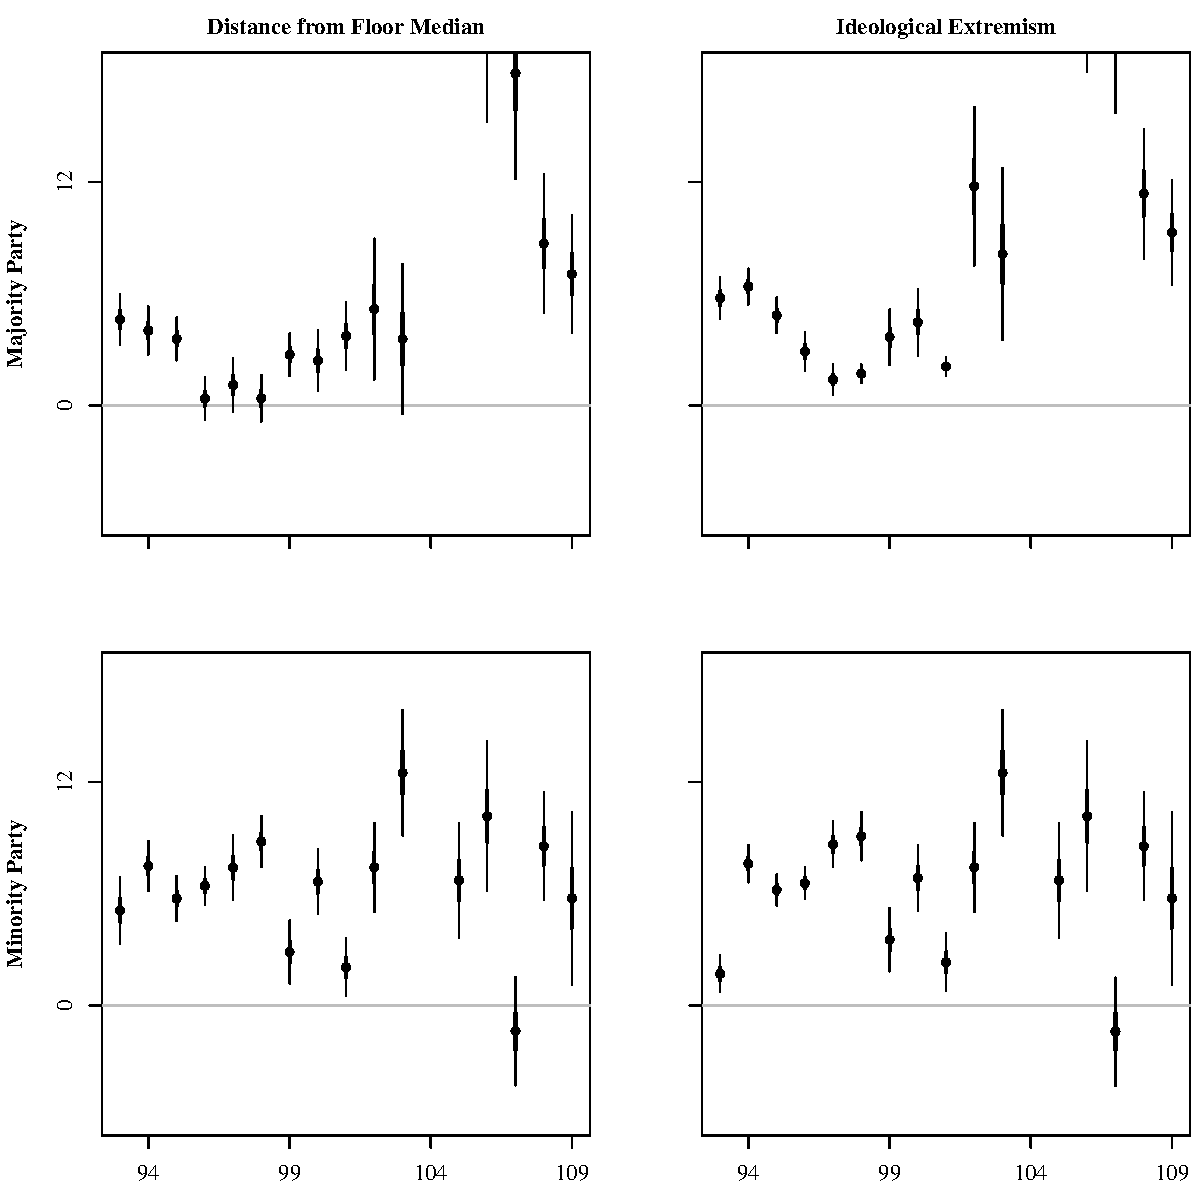
\includegraphics[width=\textwidth]{C:/Users/Ethan/Documents/GitHub/partycalls/plots/who-heeds-figure2-replication_reassign_flip_flop_votes.pdf}
	
\end{figure}
	
	
	
	
	
	
\end{document}